\documentclass[12pt, a4paper]{article}

\usepackage{amsmath}
\usepackage{amsfonts}
\usepackage{amssymb}
\usepackage{graphicx}
\usepackage{float}
\usepackage{listings}
\usepackage{rotating}
\usepackage{tikz}
\usepackage{verbatim}
\pdfgentounicode=1
\pdfmapline{+cyberb@Unicode@  <cyberbit.ttf}

\begin{document}

\title{TGAPaint}
\author{P. Baillehache}
\date{\today}
\maketitle

\tableofcontents

\section*{Introduction}

TGAPaint library is a C library to create and manipulate pictures in TGA format.\\

It offers functions to create, open and save TGA files, restricted to types 2 (uncompressed true-color image) and 10 (run-length encoded true-color image), pixel depths of 16, 24, and 32, and color map 0 (no color map) and 1 (standard TGA color map).The user can access the header and pixels values, paint simple geometric shapes (point, line, curve, rectangle, filled rectangle, ellipse and filled ellipse) or Shapoid and print text (ascii characters) with a virtual pencil (round/square shape, solid/blend color, antialias), and apply gaussian blur to the picture.\\ 

\section{Interface}

\begin{scriptsize}
\begin{ttfamily}
\verbatiminput{../tgapaint.h}
\end{ttfamily}
\end{scriptsize}

\section{Code}

\subsection{tgapaint.c}

\begin{scriptsize}
\begin{ttfamily}
\verbatiminput{../tgapaint.c}
\end{ttfamily}
\end{scriptsize}

\subsection{tgafont.c}

\begin{scriptsize}
\begin{ttfamily}
\verbatiminput{../tgafont.c}
\end{ttfamily}
\end{scriptsize}

\section{Makefile}

\begin{scriptsize}
\begin{ttfamily}
\verbatiminput{../Makefile}
\end{ttfamily}
\end{scriptsize}

\section{Usage}

\begin{scriptsize}
\begin{ttfamily}
\verbatiminput{../main.c}
\end{ttfamily}
\end{scriptsize}

Output:\\
\begin{scriptsize}
\begin{ttfamily}
\verbatiminput{../output.txt}
\end{ttfamily}
\end{scriptsize}


Resulting image (enlarge):\\
\begin{center}
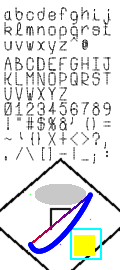
\includegraphics[width=5cm]{tga.png}
\end{center} 
	
\end{document}


